% !TEX program = xelatex
% 第 3 章“模型假设的适用范围”图（与 fig_roadmap_merged 同一套视觉规范）
% 论文中用法：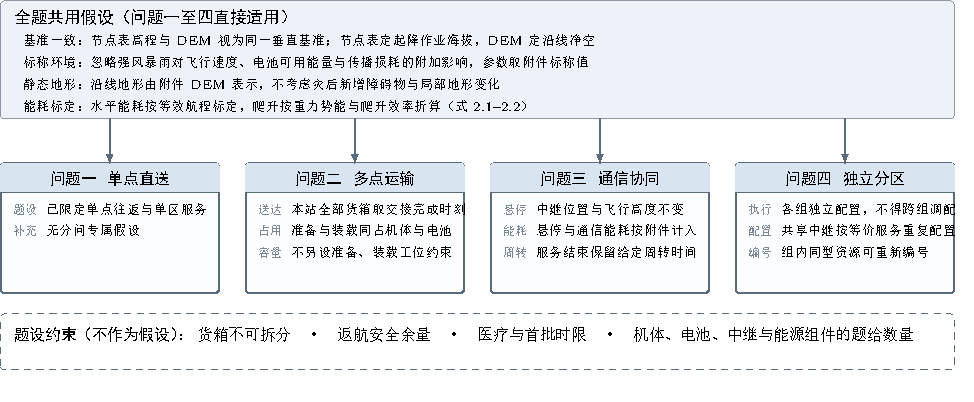
\includegraphics[width=\textwidth]{../figures/fig_assumption_scope.pdf}
\documentclass[12pt]{ctexart}
\usepackage[margin=0pt,paperwidth=16.5cm,paperheight=6.8cm]{geometry}
\usepackage{tikz}
\usetikzlibrary{arrows.meta}
\pagestyle{empty}

\definecolor{cBand}{HTML}{EDF2F8}
\definecolor{cBox}{HTML}{FCFDFE}
\definecolor{cTitle}{HTML}{D9E4F1}
\definecolor{cLine}{HTML}{5A6B7D}
\definecolor{cAccent}{HTML}{2E5C8A}
\definecolor{cRole}{HTML}{7A8794}

\newcommand{\cl}[2]{{\fontsize{6}{7.2}\selectfont\color{cRole}#1}\ \fontsize{6.5}{9}\selectfont #2}
\newcommand{\cln}[4]{\node[anchor=west,align=left] at (#1,#2) {\cl{#3}{#4}};}

\begin{document}
\noindent
\begin{tikzpicture}[x=1cm,y=1cm,every node/.style={inner sep=0pt}]

\def\bw{3.70}
\def\gap{0.45}
\def\xa{0.175}
\def\xb{16.325}

%% ================= 全题共用假设 =================
\filldraw[fill=cBand,draw=cLine!70,line width=0.4pt,rounded corners=2pt]
  (\xa,4.55) rectangle (\xb,6.55);
\node[anchor=west] at (\xa+0.22,6.28)
  {\heiti\fontsize{8}{9.6}\selectfont 全题共用假设（问题一至四直接适用）};
\node[anchor=west] at (\xa+0.22,5.88)
  {\fontsize{6.5}{8.4}\selectfont
   ①\ 基准一致：节点表高程与 DEM 视为同一垂直基准；节点表定起降作业海拔，DEM 定沿线净空};
\node[anchor=west] at (\xa+0.22,5.51)
  {\fontsize{6.5}{8.4}\selectfont
   ②\ 标称环境：忽略强风暴雨对飞行速度、电池可用能量与传播损耗的附加影响，参数取附件标称值};
\node[anchor=west] at (\xa+0.22,5.14)
  {\fontsize{6.5}{8.4}\selectfont
   ③\ 静态地形：沿线地形由附件 DEM 表示，不考虑灾后新增障碍物与局部地形变化};
\node[anchor=west] at (\xa+0.22,4.77)
  {\fontsize{6.5}{8.4}\selectfont
   ④\ 能耗标定：水平能耗按等效航程标定，爬升按重力势能与爬升效率折算（式~2.1--2.2）};

%% ================= 四个分问的题设边界与补充口径 =================
\pgfmathsetmacro{\bA}{\xa}
\pgfmathsetmacro{\bB}{\xa+1*(\bw+\gap)}
\pgfmathsetmacro{\bC}{\xa+2*(\bw+\gap)}
\pgfmathsetmacro{\bD}{\xa+3*(\bw+\gap)}

\foreach \bx/\ttl in {%
  \bA/{问题一\ \ 单点直送},%
  \bB/{问题二\ \ 多点运输},%
  \bC/{问题三\ \ 通信协同},%
  \bD/{问题四\ \ 独立分区}}{%
  \filldraw[fill=cBox,draw=cLine,line width=0.5pt,rounded corners=2pt]
    (\bx,1.60) rectangle ++(\bw,2.20);
  \begin{scope}
    \clip[rounded corners=2pt] (\bx,1.60) rectangle ++(\bw,2.20);
    \fill[cTitle] (\bx,3.30) rectangle ++(\bw,0.50);
  \end{scope}
  \draw[draw=cLine,line width=0.4pt] (\bx,3.30) -- ++(\bw,0);
  \node[anchor=center] at (\bx+\bw/2,3.55)
    {\heiti\fontsize{7.5}{9}\selectfont \ttl};
  \draw[-{Latex[length=1.5mm,width=1.1mm]},draw=cLine,line width=0.5pt]
    (\bx+\bw/2,4.55) -- (\bx+\bw/2,3.80);
}

%% 各问的补充口径
\cln{\bA+0.20}{3.02}{题设}{已限定单点往返与单区服务}
\cln{\bA+0.20}{2.66}{补充}{无分问专属假设}

\cln{\bB+0.20}{3.02}{送达}{本站全部货箱取交接完成时刻}
\cln{\bB+0.20}{2.66}{占用}{准备与装载同占机体与电池}
\cln{\bB+0.20}{2.30}{容量}{不另设准备、装载工位约束}

\cln{\bC+0.20}{3.02}{悬停}{中继位置与飞行高度不变}
\cln{\bC+0.20}{2.66}{能耗}{悬停与通信能耗按附件计入}
\cln{\bC+0.20}{2.30}{周转}{服务结束保留给定周转时间}

\cln{\bD+0.20}{3.02}{执行}{各组独立配置，不得跨组调配}
\cln{\bD+0.20}{2.66}{配置}{共享中继按等价服务重复配置}
\cln{\bD+0.20}{2.30}{编号}{组内同型资源可重新编号}

%% ================= 题设约束（不作为假设） =================
\filldraw[fill=white,draw=cLine,line width=0.4pt,dashed,rounded corners=2pt]
  (\xa,0.30) rectangle (\xb,1.25);
\node[anchor=west] at (\xa+0.22,0.90)
  {\fontsize{7.5}{9}\selectfont
   {\heiti 题设约束（不作为假设）：}\;货箱不可拆分\quad·\quad 返航安全余量\quad·\quad
   医疗与首批时限\quad·\quad 机体、电池、中继与能源组件的题给数量};

\end{tikzpicture}
\end{document}
